\section{设计思想}
% 本程序中用到的所有数据类型的定义,主程序的流程图及各程序模块之间的调用关系
\subsection{逻辑设计}
考虑到不同的图的实现都有各自的特点,而作为统一的\emph{图}来看的话,事实上他们应该具有统一性,所以在这里,我使用了C++的继承,使得不同的图拥有统一的接口,这样对于不同的实现,他们的外在表现是一致的。

\subsubsection{基类}

\begin{figure}[H]
    \centering
    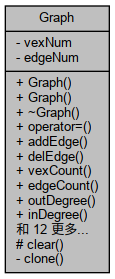
\includegraphics[width=0.1\linewidth]{figures/class_graph__coll__graph}
    \caption{Graph基类}
    \label{fig:classgraphcollgraph}
\end{figure}

\subsubsection{邻接表}

\begin{figure}
    \centering
    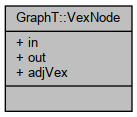
\includegraphics[width=0.5\linewidth]{figures/struct_graph_t_1_1_vex_node__coll__graph}
    \caption{顶点数据结构表}
    \label{fig:structgrapht11vexnodecollgraph}
\end{figure}

\begin{lstlisting}[language = c++]
 class GraphT : public Graph {
 public:
     explicit GraphT(unsigned long n);
     explicit GraphT(const Graph &rhs);
     void addEdge(unsigned long source, unsigned long sink) override;
     void delEdge(unsigned long source, unsigned long sink) override;
     inline unsigned long vexCount() const override;
     unsigned long edgeCount() const override;
     unsigned long outDegree(unsigned long source) const override;
     unsigned long inDegree(unsigned long source) const override;
     bool hasEdge(unsigned long source, unsigned long sink) const override;
     void foreach(unsigned long source, std::function<bool(unsigned long, unsigned long)> &func) const override;
     void reset() override;
     void reset(unsigned long vexNum) override;
 private:
     void clear() override;
     typedef struct VexNode {
              unsigned long in;
         unsigned long out;
         std::forward_list<unsigned long> adjVex;
     } VexNode;
     std::vector<VexNode> vexes;
 };
\end{lstlisting}

\subsubsection{邻接矩阵}

\begin{lstlisting}[language = c++]
class GraphM : public Graph {
public:
     explicit GraphM(unsigned long n);
     explicit GraphM(const Graph &rhs);
     void addEdge(unsigned long source, unsigned long sink) override;
     void delEdge(unsigned long source, unsigned long sink) override;
     inline unsigned long vexCount() const override;
     unsigned long edgeCount() const override;
     unsigned long outDegree(unsigned long source) const override;
     unsigned long inDegree(unsigned long source) const override;
     bool hasEdge(unsigned long source, unsigned long sink) const override;
     void foreach(unsigned long source, std::function<bool(unsigned long, unsigned long)> &func) const override;
     void reset() override;
     void reset(unsigned long vexNum) override;
 private:
     void clear() override;
     std::vector<std::vector<bool>> vexes;
 };
\end{lstlisting}

\subsubsection{十字链表}

\begin{figure}[H]
    \centering
    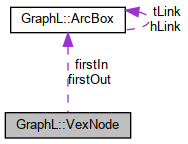
\includegraphics[width=0.2\linewidth]{figures/struct_graph_l_1_1_vex_node__coll__graph}
    \caption{顶点及弧结构}
    \label{fig:structgraphl11vexnodecollgraph}
\end{figure}

\begin{lstlisting}[language = c++]
 class GraphL : public Graph {
 public:
     explicit GraphL(unsigned long n);
     explicit GraphL(const Graph &rhs);
     ~GraphL() override { clear(); };
     void addEdge(unsigned long source, unsigned long sink) override;
     void delEdge(unsigned long source, unsigned long sink) override;
     unsigned long vexCount() const override;
     unsigned long edgeCount() const override;
     unsigned long outDegree(unsigned long source) const override;
     unsigned long inDegree(unsigned long source) const override;
     bool hasEdge(unsigned long source, unsigned long sink) const override;
     void foreach(unsigned long source, std::function<bool(unsigned long, unsigned long)> &func) const override;
     void foreachIn(unsigned long dst, std::function<bool(unsigned long, unsigned long)> &func) const;
     void reset() override;
     void reset(unsigned long vexNum) override;
 private:
     typedef struct ArcBox {
         unsigned long headVex, tailVex;
         struct ArcBox *hLink, *tLink;
         ArcBox(unsigned long head, unsigned long tail, ArcBox *headLink, ArcBox *tailLink) :
             headVex(head), tailVex(tail), hLink(headLink), tLink(tailLink) {}
     } ArcBox;
 
     typedef struct VexNode {
         unsigned long in, out;
         ArcBox *firstIn, *firstOut;
         VexNode() : in(0), out(0), firstIn(nullptr), firstOut(nullptr) {};
     } VexNode;
 
     void clear() override;
     std::vector<VexNode> vexes;
 };
\end{lstlisting}
\subsection{整体依赖关系图}

\begin{figure}[H]
    \centering
    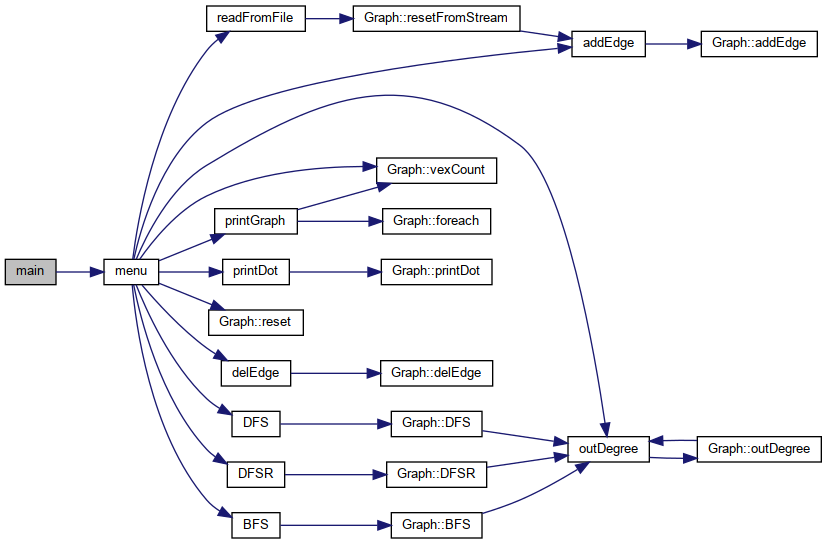
\includegraphics[width=0.6\linewidth]{figures/_graph_main_8cpp__incl}
    \caption{依赖关系图}
    \label{fig:graphmain8cppincl}
\end{figure}


\subsection{Main函数流程图}

\begin{figure}[H]
    \centering
    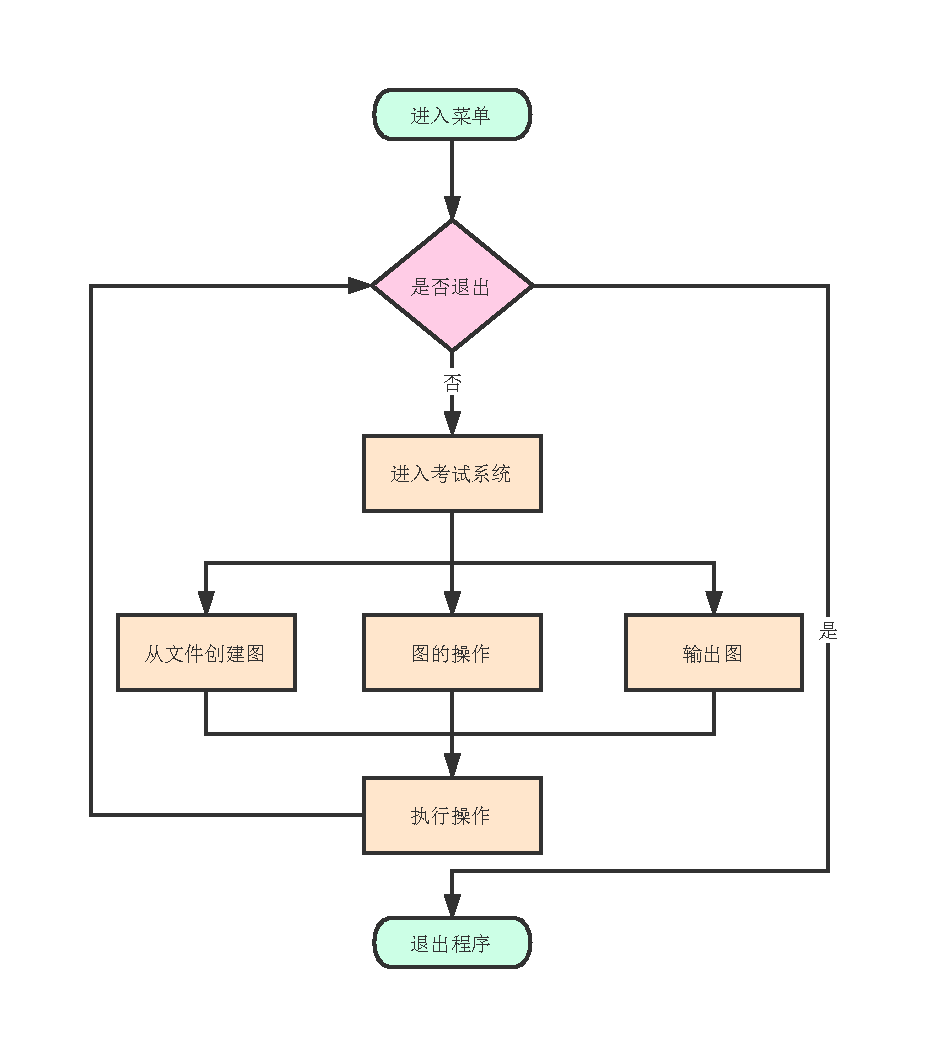
\includegraphics[width=0.6\linewidth]{figures/flowchart}
    \caption{程序流程图}
    \label{fig:flowchart}
\end{figure}

